% M. S. Tsoeu (2011), University of Cape Town <mohohlo.tsoeu@uct.ac.za>

% This is a project report templace document created for EEE4022FS students at the University of Cape Town.
%
% This file should be is processed with ``pdflatex`` and might need a few modifications if a different processor is chosen.


\documentclass[a4paper,12pt]{report}

%Include packages you need to use here

\usepackage[top = 1in, bottom = 1in, left = 1in, right = 1in]{geometry}
\usepackage{graphicx}
\usepackage{fancyhdr}
\usepackage{amsmath, amsthm, amssymb}
\usepackage{lastpage}
\usepackage{subfigure}
\usepackage{lscape}
\usepackage{hyphenat}
\usepackage{setspace}
\usepackage{hyperref}
\usepackage{float}
\usepackage{gensymb}
\usepackage{caption} %my addition
\usepackage{mathtools} %my addition
\usepackage[framed,numbered,autolinebreaks,useliterate]{mcode} % load package with ``framed'' and ``numbered'' option. - my addition for matlab code in listings
\usepackage{pdfpages} %for including ethics form

%c code style for latex
\input{ccode}
%/c code style for latex

%\usepackage{bibtex}

% Include page formatting here. 
\parskip = 6mm
\parindent = 0mm
\renewcommand{\headrulewidth}{0pt}
\rhead[]{\thesection}
\lhead[\thechapter]{}


\begin{document}

% This section formats the title page of the Report.
\thispagestyle{empty}
{\Huge \begin{center}
% Modify the line below to insert your title.
Laser Tag using Narrow Beam Infrared Radiation
\hrule 
% Modify the line below to insert your subtitle.
{\Large An Investigation into Hardware and Software Requirements}
\end{center}}

\vskip 5mm
\begin{center}
\- \- \- \- \- \- \- \- \- \-\includegraphics[scale = 0.3]{figures/template/uctLogo.png}
\end{center}

\vskip 5mm
\begin{center}
Presented by:\\
Justin Michael Wylie		% Insert your name here
\end{center}

\vskip 10mm
\begin{center}
Prepared for:\\
Dr. Simon Winberg\\ 		% Insert your supervisor's name here.
Dept. of Electrical and Electronics Engineering\\University of Cape Town
\end{center}


\vskip 10mm
\begin{center}
Submitted to the Department of Electrical Engineering at the University of Cape Town in partial
fulfilment of the academic requirements for a Bachelor of Science degree in Electrical and Computer Engineering

\end{center}


\vskip 5mm
\begin{center}{\bf \today}
\end{center}

\newpage
\thispagestyle{empty}
\mbox{}
\newpage

\onehalfspacing
\nohyphens{
\thispagestyle{empty}
\vskip 40mm


% Please leave the declaration as it is (Standard UCT declaration).
{\Large Declaration}\\
\hrule

\vskip 10mm
\begin{enumerate}
\item I know that plagiarism is wrong. Plagiarism is to use another's work and pretend that it is one's
own.
\item I have used the IEEE convention for citation and referencing. Each contribution to, and quotation in,
this report from the work(s) of other people has been attributed, and has been cited and
referenced.
\item This report is my own work.
\item I have not allowed, and will not allow, anyone to copy my work with the intention of passing it off
as their own work or part thereof.
\end{enumerate}
\vskip 10mm
Signature:\ldots\ldots\ldots\ldots\ldots\ldots\ldots\ldots\ldots 
\\J. M. Wylie 		% Chante this line to your name.
\vskip10mm
Date:\ldots\ldots\ldots\ldots\ldots\ldots\ldots\ldots\ldots\ldots .


\fancyfoot[C]{\thepage}
\pagestyle{plain}
\newpage
\pagenumbering{roman}
{\Large Acknowledgments}\\
\hrule

%todo acknowledgements
%I would like to express my gratitude to the many people who have played a role in supporting and guiding me throughout the course of this investigation.


\textbf{Dr Simon Winberg}, for his continued supervision and guidance throughout the project.

\textbf{Justin Pead}, for helping me source components and for the insightful discussions around analog circuit design.

\textbf{My Family}, for their encouragement and support. A special mention to my parents for their help proof reading my report.

\textbf{My Friends}, for their genuine friendship and support. A special mention to Stefan who came out to help me move the target while I was performing the late evening range test and to Amy for the help proof reading my report.

\textbf{Engineering Class Mates}, a special mention to Callum, Kate, Matthew and Thomas for the countless hours spent in the virtual library on Discord.

\textbf{The Lord}, for his provision and the opportunity to study at UCT.




\newpage

{\Large Abstract}\\
\hrule

% Place your abstract here.
%\begin{itemize}
%\item Abstract is written here
%\end{itemize}

%NB: this is going to be read through!
Laser Tag is a light-based electronic sport, popular amongst juveniles and enjoyed by persons of all ages. The technology used in laser tag sports systems has not seen much innovation over the years with most systems still requiring large cumbersome vests and a specialized arena.

This investigation focuses on the central component of laser tag systems, the uni-directional communication via a narrow beam of IR light. This poses a unique engineering design problem due to the high directionality requirement along with size, weight, and cost constraints.

This project approaches the engineering problem by it breaking down into fine-grained sub-problems, designing solutions for these sub-problems, and finally implementing and analysing the performance of these modules and the system as a whole.

%todo: improve this paragraph
At the centre of this project is the design, realization and analysis of an infrared-based line-of-sight communication system. This investigation aims to provide insight into the components of such a system through the thorough analysis of modules as well as document what kind of performance can be achieved on a limited budget in terms of range and tolerance to ambient lighting.

%todo: must cover WHAT the results are!


%A breakdown of the project methodology follows the literature review. The design phase is then documented, during which subsystems are identified and designed. Following the design phase, the modules are realized and experimentally evaluated. During the final phases of this project, the results are analysed and conclusions are drawn.


\iffalse
Your abstract provides a good idea of where the project is going, however, it's missing your key findings and conclusion. An abstract is a highly condensed summary of the entire project and usually follows the following format: intro and problem, project aim, methods, key findings and conclusion.

The abstract is usually the most difficult part to write because of how condensed it needs to be. If you need inspiration, have a look at the abstracts of relevant journal articles :)
\fi

\newpage
\tableofcontents

%\newpage
%\listoffigures

%\newpage
%\listoftables

% Page formatting, to place section titles as headers of odd pages and Chapter titles as headers of even pages.
\newpage
\fancyhead[RE,LO]{}
\fancyhead[LE]{\leftmark}
\fancyhead[RO]{\rightmark}
\pagestyle{fancy}

\pagenumbering{arabic}

% THe files included below are .tex files containing the respective chapters these are already created in this package and you can add to or modify them.
\chapter{Introduction}

\section{Background to the study}
%A very brief background to your area of research. Start off with a general introduction to the area and
%then narrow it down to your focus area. Used to set the scene \cite{Knight2013}.
Since the discovery of infrared (IR) light by William Herschel in the 1800s \cite{Rowan-Robinson2013}, it has found application in technologies ranging from military grade night vision equipment to the humble television remote.

On the electromagnetic spectrum infrared radiation is just below visible light with a slightly longer wavelength. Being invisible to the naked eye while retaining much the same behavioural properties as visible light is one of the reasons it has so many useful applications.

This study focuses on the application of IR in the recreational sport of laser tag. Although many use cases of infrared involve passive observation, this investigation seeks to understand appropriate means to generate and detect a narrow infrared beam for the purposes of unidirectional communication.

Much is known about the use of infrared in remote controls, but less information is available on the specialized use of infrared in the laser tag context. This introduces several factors and constraints which are unpacked and addressed.



\section{Objectives of this study}
\subsection{Problems to be investigated}
%Description of the main questions to be investigated in this study...
An appropriate protocol for encoding information into an infrared beam needs to be developed. An investigation into the current industry-standard protocols will be performed and an appropriate protocol selected and modified to satisfy problem constraints.

An instigation into the process of generating a narrow angle beam of IR is to be investigated. This is to ensure that a measure of skill and accuracy is required in order for the player to hit the target. Techniques will be evaluated on their cost, robustness and size.

An appropriate sensor module must be developed to act as a wide angle receiver. Choosing an appropriate photo diode for this module will involve a comparison of various available options. Experiments will be performed to determine the cost vs performance of these sensors.

The investigation will also broadly cover the selection of an appropriate microcontroller and the design of various modules which will be combined into the experimental setup.

\subsection{Purpose of the study}
%Give the significance of investigating these problems. It must be obvious why you are doing this study
%and why it is relevant.
Because of the niche nature of this application specific investigation, there is little to no sources of information available that formally document the development of a recreational laser tag system.

The purpose of this study is therefore to investigate the critical components of such a system, with the goal of providing a comprehensive understanding of how the various block of such a system can be most efficiently brought together and optimized. 

\section{Scope and Limitations}
Scope indicates to the reader what has and has not been included in the study. Limitations tell the
reader what factors influenced the study such as sample size, time etc. It is not a section for excuses as
to why your project may or may not have worked.

\section{Plan of development}
Here you tell the reader how your report has been organised and what is included in each
chapter.

{\bf I recommend that you write this section last. You can then tailor it to your report.}

\chapter{Literature Review}
\label{ch_literature}

Once upon a time engineers and researchers believed... In this area of research, they used the following methods... \cite{Knight2013}

Write this section first as it will take you the longest. I suggest you start writing this as soon as you
have done your initial research at the beginning of your project. You can then return to it once you
have completed your work to edit and adjust it.

A literature review forms the theoretical basis of your project. You need to read a large number of
journal papers, sections in books, technical reports etc. relevant to your work at the start of project.
This will give you a good idea of the field of research.

When writing your review start of with the general concepts and move to the more specific aspects
explaining the necessary theory as you go. This section is NOT a copy and paste from others work or a
rewrite-but-change-one-word section. I suggest you read all your material, and then put it down and
write this section, referring back to the work only when you need to check something.

See your PCS textbook for more details on how to write a literature review.

If you include a figure or a table in your text please see the example in Fig. \ref{fig:model} as to how to caption it.
Please make sure that all text in your figures is readable and that you reference your figures if they are
from another source.

\begin{figure}[ht]
	\centering
	\includegraphics[width=0.7\textwidth]{figures/template/model.png}
	\caption{A block diagram illustrating the connections to the IRQ pin on the MCS08GT16A microcontroller (Please
	note that your headings should be short descriptions of what is in the diagram not simply the figure title)}
	\label{fig:model}
\end{figure}

%%%%%%%%%%%%%%%%%%

\section{Optics}

\subsection{Brief History}
Optics as defined by the Oxford English Dictionary is "The branch of physics that deals with the properties and phenomena of visible light (and by extension other forms of electromagnetic radiation), sometimes esp. in relation to sight." \cite{oed}.

For most of human history, little was known of the complex phenomena we call light. The first attempts to understand the properties of light were philosophical and history tells us that the Greek philosophers took interest in the subject. Around 300BC Euclid postulated that light propagated in a rectilinear fashion. He also stated the law of reflection. These principles still form part of our understanding of light today. \cite{Vohnsen_2004}

Well before any established scientific theories existed, lenses and their optical properties have been used for visual aid both for visually impaired persons and for magnification of objects. It was however only in the 17th century that the first record of telescopes can be found. Galileo is the first to record the use of such devices for the purpose of scientific inquiry.

In the 17th century scientist Descartes recorded his corpuscular theory of light. This theory was supported and further developed by Newton. In the same century Snell developed what we now know as Snell's law of refraction.

TBC.

\subsection{Optical Communication}

Optical communication concerns all manors of communicating information from one party to another through the medium of light. This investigation focuses on the use of light as a means of communication between electronic systems, however it is worth noting that optical communication certainly exist outside of this category.


\subsection{IR Communication}
This is where I talk about different IR protocols

\subsection{Materials Interaction}
This is where I talk about materials that block visible light but let IR through

%%%%%%%%%%%%%%%%%%

\section{Reliable Communication}

\subsection{Noise in Air}
Talk about interference and noise due to ambient light

\subsection{Modulation}
Talk about modulation to allow for easy detection

\subsection{Manchester Encoding}
Manchester Code is a type of phase encoding. It is classified as a line code and is produced by generating patterns through some measurable phenomena. The commonly used mediums to represent a Manchester encoded signal would be voltage, current and light (electromagnetic radiation).

Manchester coding, as its name suggests, was developed at the University of Manchester and it was first published in 1949 \cite{Jameel2019}. Manchester encoding is a protocol for integrating the clock and data into a single sequence consisting of only two symbols. It does not require clock synchronization, only that a predefined bit-width is known by both the receiver and transmitter. 

The principle behind Manchester code is to encode the information into transitions between two symbols. This technique makes the encoding scheme particularly useful in communication by means of inductive coupling such as in RFID. Due to its self-clocking property and simplicity it is the standard means of encoding for many IR applications. Perhaps the most common application is in the remote controls we use for various appliances.

Manchester code is a special form of binary phase shift keying (BPSK). A square wave of a particular frequency is chosen as the carrier and binary information is encoding by adjusting the setting a phase off set to either 0\degree or 180\degree s. In figure \ref{fig:manchesterencoding} the process of encoding 10 bits is illustrated. Two conventions exist, their difference lies solely in the definition of which logic values are represented by each of the two transitions. The convention used throughout this investigation is in accordance to the IEEE 802.3 standard which defines a logical 1 as the transition from 0 to 1 and a zero as 1 to 0. The other convention used by inventor G.E. Thomas is the inverse of this and is also widely used.\\

\begin{figure}[H]
	\centering
	\includegraphics[width=0.7\linewidth]{figures/litreview/manchester_encoding}
	\caption{Manchester code example using 10 bits}
	\label{fig:manchesterencoding}
\end{figure}

\subsubsection{Encoding Algorithm}


\subsubsection{Decoding Algorithm}
Different techniques have been developed to decode Manchester encoded sequences. In his paper on methods for decoding Manchester code, R. A. Dobre discusses an elegant and widely used finite state machine approach which has been illustrated in figure \ref{fig:manchesterdecodingfsm} below. \cite{Dobre2014}

\begin{figure}[H]
	\centering
	\includegraphics[width=0.7\linewidth]{figures/litreview/manchester_decoding_fsm.png}
	\caption{FSM Algorithm for Decoding Manchester Sequences}
	\label{fig:manchesterdecodingfsm}
\end{figure}

The state machine approach is particularly useful because it only considers the time period between the current detected edge and the previous edge. It removes the need to track samples saving on memory and reducing processing power requirements, all without introducing additional complexity.

It should be noted that this FSM assumes the first bit transmitted is always a logical 1. In addition does not detect the end of a sequence, so additional logic is required such as a counter to detect when a certain number of bits have been received or by means of implementing timeout detection.


\subsection{Error Control}

In information theory, error control is the field of study that concerns issues of detecting errors in digital communications and in certain instances provides the means to corrected these errors. Whenever data is transmitted over some kind of network, there is the possibility that interference can cause a bit to flip resulting in an error. Richard Hamming pioneered in the development of digital error control and is known for (amongst other things) the Hamming code.

\subsubsection{Methods}
Various ways to detect and potentially correct the presence of an error. The most trivial technique known as a 'repetition code' simply involves sending the information three times, making it possible to detect if one of the three data-streams doesn't match the others. Although repetition codes allows for both error detection and correction, it is horribly inefficient. Various techniques have been developed and each technique balances complexity and efficiency.

\subsubsection{Hamming Code}


\subsection{Demodulation}
Need to talk about demodulating, Goertzel, DSP, tone-detectors


%%%%%%%%%%%%%%%%%%

\section{IR Radiation}
This is where I talk about the section of the EM spectrum that is IR


\subsection{IR Radiation Detection}

Photodiodes and transistors




%%%%%%%%%%%%%%%%%%

\section{Recreational Electronics}


\subsection{Recreational Laser Use}

\section{Microcontrollers}
Histroy of how uc have come down in price making them a viable component in hobby electronics.

\subsection{ADC}

\subsection{Timers}
PWM

\subsection{Libraries - The HAL Library}


%%%%%%%%%%%%%%%%%%

\section{Pulse Width Modulation}








\chapter{Methodology}
\label{ch_methodology}

%This is what I did to test and confirm my hypothesis.


%You may want to split this chapter into sub chapters depending on your design. I suggest you change
%the title to something more specific to your project.

%This is where you describe your design process in detail, from component/device selection to actual
%design implementation, to how you tested your system. Remember detail is important in technical
%writing. Do not just write I used a computer give the computer specifications or the oscilloscopes part
%number. Describe the system in enough detail so that someone else can replicate your design as well
%as your testing methodology.

%If you use or design code for your system, represent it as flow diagrams in text.

\section{Outline}

This study set out to investigate the performance of modules created for a uni-directional data link in the context of laser tag systems. The following chapter presents the methodology that was followed throughout the investigation. A phased approach was taken and the following chapter gives a break down of those phases.

\begin{figure}[H]
	\centering
	\includegraphics[width=0.5\textwidth]{figures/methodology/methodology}
	\caption{Methodology Flow Diagram}
	\label{fig:methodology_overview}
\end{figure}

%todo: this will need re-wroking after finilized the flow diagram
The first phase involves investigating the relevant literature. The second phase involves identifying and designing the modular subsystems, this phase of the project incorporates a portion of feedback from the incremental stage. The third phase is the experimental setup during which experiments are devised and test/measurement equipment selected. Following the experimental setup is an iterative stage which comprises phase four and five. During phase four the modules are developed according to the designs produced in the second phase. Phase five then involves performing the experiments devised in the third phase to evaluate the modules.

The experimentation phase loops back to the development stage illustrating that some experiments were performed progressively as modules are realized. Following the design paradigm of the spiral model, a feedback path from the incremental stage back to the design exists to illustrated that certain design choices were made based on the experimental results.

During phase 7 the results are compiled and analysed. During the 8\textsuperscript{th} phase these results are interpreted and conclusions are drawn bringing closure to the research project.


%todo: the following sections are very 'outdated'/incomplete
\section{Phase 1 - Literature}

During the first phase of the project, the relevant literature is reviewed. The objective of this phase is to determine the various techniques that have been established in the field of optical communication. For each of the topics a broad overview is presented, followed by a detailed review of specific concepts and theories.

The design and evaluation of a complex communication system involves reviewing theory in various areas and the following questions served as a guide for surveying the available literature.

%todo: consider improving these questions
\begin{itemize}
	%\item What are current examples of uni-directional communication systems?
	\item How might non-laser light be focused into a narrow beam? %Optics
	\item What properties make infrared light useful? %Optics
	\item What methods exist for detection of light? %Detection of Raditation
	\item What techniques exist for reliable communication? %Reliable Communication
	\item What techniques exist for the purpose of tone detection? %DSP &Analog processing
	%an item on filtering and pre-dsp stuff?
\end{itemize}

The literature review is presented in chapter \ref{ch_literature}.

%%%%%%%%%%%%%%%%%%%%

\section{Phase 2 - Design}

The design phase of this investigation is dedicated to the development of the individual modules and software algorithms. This phase begins with a decomposition of the uni-directional communication system into a set of modules. Figure \ref{fig:designoverview} provides a high-level overview of the system decomposition.

\begin{figure}[H]
	\centering
	\includegraphics[width=0.7\linewidth]{figures/methodology/design_overview}
	\caption{Design Overview}
	\label{fig:designoverview}
\end{figure}

The second phase is documented in chapter \ref{ch_design}. For each module a brief description of the purpose and required functionality of the module is given. The design of module is then presented, including important calculations, circuit schematics and relevant diagrams where appropriate. For each module an image of the final implementation is also shown.

Throughout the design phase, various simulations were used to predict the behaviour of algorithms\footnote{Octave was used to validate algorithms} and circuits\footnote{LTSpice was used to simulate circuits}.

%%%%%%%%%%%%%%%%%%%%

\section{Phase 3 - Development and Realization}

The third phase concerns the development of the individual modules. During this phase each module was realized according its design.

Modules were first implemented on a breadboard to confirm valid behaviour. In the case of a failed implementation due to a design oversight the design was reworked, this is illustrated using a dotted feedback path from phase 3 to phase 2 in figure \ref{fig:methodology_overview}. Only the final module design and implementation has been documented in the body of this report.

With the exception of the STM32 development boards, all the module designs were implemented on strip-board. The use of PCB was avoided due to uncertainty caused by the COVID-19 epidemic.

%%%%%%%%%%%%%%%%%%%%


\section{Phase 4 - Experimental Setup}

The fourth phase is the experimental set-up. This phase outlines the procedure followed to setup the test and measurement equipment and the module or collection of modules for the purposes of performing experiments and gathering empirical data. Chapter \ref{ch_experimentation} is dedicated to the procedures followed for each experiment.

Due to the unique functionality of each module, it is necessary to use different experimental setups to evaluate different modules. Hence phase four forms part of an \textit{iterative stage} which is used to illustrate that for various phases of experimentation, a unique experimental setup has been devised.

Equipment used throughout this investigation is documented at the end of this chapter in section \ref{sec:test_and_measurement_equipment}


%%%%%%%%%%%%%%%%%%%%



\section{Phase 5 - Experimentation}

Phase five concerns the execution of the experiments outlined in chapter \ref{ch_experimentation} and forms the second half of the \textit{iterative stage}. During this phase, the experiments are executed and the results are prepared for analysis.

The objective of the experimentation phase is to provide results that may be used to gain insight into each module's performance. Results will consist primarily of empirical results, but in certain cases also include simulation results.

The results gathered during the experimentation phase are documented in chapter \ref{ch_results}.

%%%%%%%%%%%%%%%%%%%%

\section{Phase 7 - Analysis of Results}

The seventh phase of this investigation is the analysis of results gathered during the experimentation. The objective of this phase is to interoperate the results and draw insights.

During this phase, the performance of the individual modules is evaluated. Brief reasoning is provided where the results do not align with the theorised outcome.

%todo: confirm this is the structure
The analysis for each set of results has been place in chapter \ref{ch_results}. This has been done to increase readability.


%%%%%%%%%%%%%%%%%%%%

\section{Phase 8 - Discussion and Closure}

%todo: improve this section after completing phase 8
In this final phase of the project, the results and analysis of the results are discussed in the greater context of the research questions. The discussion will comment on the effectiveness of each of the modules. 

Discussion is bought to a close with a comment on the  proposals for further research.



%%%%%%%%%%%%%%%%%%%%

\section{Test and Measurement Equipment}
\label{sec:test_and_measurement_equipment}









\chapter{Design}
\label{ch_design}

This chapter is dedicated to the various modules which comprise the laser tag system being investigated. The system is complex and comprises of many modules both in hardware and software. An overview of the entire system is given followed by the design of the individual modules.

It is important to reiterate at this point that this study aims determine the core components of a laser tag module with respect to the tagger and target system. The goal is not to design a ready to play 'user friendly' kit, but rather to determine what modules are required in such a system and how these components perform through the execution of various experiments.

\section{System Overview}

The hardware and software modules of the system will be addressed separately. Figure \ref{fig:system_overview_hardware} gives an overview of the hardware modules required to create a functional laser tag system.

\subsection{Hardware}

\begin{figure}[H]
	\centering
	\includegraphics[width=0.9\textwidth]{figures/design/system_overview_hardware}
	\caption{Block Diagram of Hardware Modules}
	\label{fig:system_overview_hardware}
\end{figure}

\subsubsection{Tagger}
The tagger system, in terms of hardware, comprises of a main processor which has been realised on the UCT STM32\footnotemark{} development board. The main processor communicates with the carrier frequency generation module which is responsible for producing the 36kHz square waveform which feeds into the final hardware module of the tagger, the LED driver. Two led driver modules have been design, they both accept the same input signal and are identical in their purpose. The difference between the two modules is in the rated output power, the low power module is designed to drive a typical IR led while the high power module has been designed to drive a high power 3W IR led.

\footnotetext{STM32F051C6}

\subsubsection{Target}
The target system comprises many more hardware modules, this is due to the comparably higher complexity involved in detecting and processing signals. An additional module is also required to allow for a comparison between using a photodiode versus a phototransistor, as these each require a custom dedicated hardware module. The target system hardware consists of three IR sensors, in addition to the two sensors just mention, an 'all in one' IR receiver device was used to act as a golden measure against which to test the other two receivers. The output of the IR receiver module can be routed directly to the target main processor.

The outputs of the photodiode and phototransistor IR detection modules are routed into a signal conditioning module. This module performs anti-alias filtering and rectification of the signal, this is to ensure the signal is within the specifications of the tone detector. The tone detection modules comprises of a digital signal processing (DSP) algorithm, implemented on an STM32 MPU. The output of the tone detection module may be routed to the target main processor. The target main processor is implemented on the UCT STM32 development board.

\subsection{Software}

\begin{figure}[H]
	\centering
	%\includegraphics[width=0.9\textwidth]{figures/design/system_overview_hardware}
	\caption{Block Diagram of Software Modules}
	\label{fig:system_overview_software}
\end{figure}



\section{Hardware Modules}

\subsection{Tagger \& Target MCUs}
%Missing
% - Schematic and the like in the appendix
The laser tag systems has two main processors. One for the tagger and another for the target. The hardware used for main processor in each case is the UCT development board built around the STM32F051C6 microcontroller.

\begin{figure}[H]
	\centering
	\includegraphics[width=.5\textwidth]{figures/design/dev_board_image.jpg}
	\caption{UCT STM32 Development Board}
	\label{fig:stm32_dev_board}
\end{figure}

The development board provides break-out pins for the microcontroller, 4 input buttons, an array of 8 LEDs, an LCD display and a built-in st-link v2 for debugging and programming the processor. 


\subsection{Carrier Frequency Generator}
%Missing
% - Calculations and chosen values
To generate the 36kHz carrier waveform the LM555 timer IC was used. The module is designed to receive a 3.3V logic control signal. The LED driver modules were designed to operate using an open-drain control signal, therefore a transistor was used to convert the push-pull output to an open-drain output. In addition, transistors were used to convert the 3.3V control signal to a 5V input for the RST pin. Figure \ref{fig:schematic_carrier_generation} shows the schematic for the module.


\begin{figure}[H]
	\centering
	\includegraphics[width=.8\textwidth]{figures/design/carrier_waveform_generator_555.JPG}
	\caption{Carrier Generation Module Schematic}
	\label{fig:schematic_carrier_generation}
\end{figure}

According to the data sheet the period my be calculated as \(T = 0.693 (R_2 + 2R_3) C1\). A capacitor value of 10nF was chosen. Therefore, to generate a waveform with the desired period of $27.7\mu S$ the required theoretical value of $(R_2 + 2R_3)$ is $4k\Omega$.
%todo: finnish explaining resistor choice

%todo: finnish this paragraph
%After testing
The above design was implemented on a breadboard to test the


\begin{figure}[H]
	\centering
	\includegraphics[width=.6\textwidth]{figures/modules/carrier_generator.jpg}
	\caption{Carrier Generation Module}
	\label{fig:module_carrier_generation}
\end{figure}

\subsection{Power LED Driver}
%Missing:
% - Specs and component choice etc.

To operate the 3W high power IR LED a constant current driver module needed to be implemented. Because the LED needs to be modulated at 36kHz, standard LED drivers that use a switching regulator are not viable because the switching frequency requirements exceed those available in standard ICs.

\begin{figure}[H]
	\centering
	\includegraphics[width=.8\textwidth]{figures/design/power_led_driver.JPG}
	\caption{Power LED Driver Module Schematic}
	\label{fig:schematic_power_led_driver}
\end{figure}

Instead a linear regulator was designed. Figure \ref{fig:schematic_power_led_driver} shows the design of a high power linear regulator, built around the IRLZ44 enhancement PMOSFET. Heat-sinks where attached to both the high power LED and the IRLZ44 power MOSFET. However because the LED is only on for short bursts spread over sufficiently long time intervals it is likely that the heat-sinks are unnecessary.

The module is designed to be driven by an open-drain configured GPIO pin. By pulling the control signal low, the LED is powered and when the control signal is left floating the LED is powered off.

\begin{figure}[H]
	\centering
	\includegraphics[width=.6\textwidth]{figures/modules/power_led_driver.jpg}
	\caption{Power LED Driver Module}
	\label{fig:module_power_led_driver}
\end{figure}

\subsection{Power LED Focus System}
%Missing:
% - ...

The high power IR LED has a wide beam angle, as it is designed for large area illumination. This is the opposite effect that is desired for a laser tag system. To rectify this, a focus system in the form of a light focusing tube was designed. This prevents light from spilling out the side and it focuses the beam to minimize dispersion over long distances.

\begin{figure}[H]
	\centering
	\includegraphics[width=.8\textwidth]{figures/design/beam_tube.png}
	\caption{Exploded View - Light Focusing Tube}
	\label{fig:light_focusing_tube}
\end{figure}

Figure \ref{fig:light_focusing_tube} above shows the components used to construct the light focusing tube. The length $l_{pipe}$ was determined by summing the experimentally calculated focal length of the lens with the length $l_{lens}$. Included in the calculation of the pipe length was the non-zero thickness of the light-seal (made out of 3mm hard-board) and the 3mm length of lens that remained external to the PVC piping.

The 40mm PVC piping used had a wall thickness of 2.3mm resulting in an inner diameter of 37.7mm. The magnifying lens had a length of 30mm and the lens is in-set by 1mm. The experimental result from section \ref{exp:focal_length} showed the focal length of the magnifying lens to be 53mm.

The length $l_{pipe}$ was calculated as follows

\[l_{pipe} = l_{lens} - l_{lens\_external} + l_{focal} - l_{light\_seal\_thickness} + l_{lens\_in-set\_distance}\]
\[l_{pipe} = 30mm - 3mm + 53mm - 3mm + 1mm = 78mm\]


\begin{figure}[H]
	\centering
	\includegraphics[width=.6\textwidth]{figures/modules/light_focus_tube_lens.jpg}
	\caption{Light Focus System}
	\label{fig:module_light_focus}
\end{figure}

\subsection{LED Driver}
%Missing:
% - Specs and component choice etc.

Due to the high power demands of the 3W IR LED, it is much more appropriate to perform test and develop the communication protocol using a low power IR led. A driver module was designed for this specific purpose.

\begin{figure}[H]
	\centering
	\includegraphics[width=.6\textwidth]{figures/design/low_power_led_driver.JPG}
	\caption{Low-Power LED Driver Module Schematic}
	\label{fig:schematic_low_power_led_driver}
\end{figure}

Figure \ref{fig:schematic_low_power_led_driver} shows the schematic for this driver module. The module is designed to be driven using an open-drain configured GPIO pin so that it is 'drop-in' compatible with the high power driver module.


\begin{figure}[H]
	\centering
	\includegraphics[width=.6\textwidth]{figures/modules/led_driver.jpg}
	\caption{LED Driver Module}
	\label{fig:module_led_driver}
\end{figure}

\subsection{Photodiode IR Detector}
%Missing:
% - Schematic and explaination
% - Talk about MCP6022 and important specs

The photodiode IR detector module is designed to detect changes in infrared radiation and convert these fluctuations into a voltage signal.

\begin{figure}[H]
	\centering
	\includegraphics[width=.8\textwidth]{figures/design/photodiode_transimpedance.JPG}
	\caption{Photodiode IR Detector Module Schematic}
	\label{fig:schematic_photodiode_transimpedance}
\end{figure}

The circuit shown in figure \ref{fig:schematic_photodiode_transimpedance} is designed to produce a voltage in proportion to the current flowing through the photodiode. The circuit is inspired by S. Schrires 'Infrared Radio Link' circuit which is found in the EEE3071 course notes\cite{Schrire2007}.


\begin{figure}[H]
	\centering
	\includegraphics[width=.6\textwidth]{figures/modules/photodiode_receiver.jpg}
	\caption{Photodiode IR Receiver Module}
	\label{fig:module_photodiode_receiver}
\end{figure}

\subsection{Phototransistor IR Detector}
%todo:
% - Schematic and explaination


The phototransistor IR detector module is designed to detect changes in infrared radiation and convert these fluctuations into a voltage signal.

\begin{figure}[H]
	\centering
	\includegraphics[width=.6\textwidth]{figures/modules/phototransistor_receiver.jpg}
	\caption{Phototransistor IR Detector Module}
	\label{fig:module_phototransistor_detector}
\end{figure}

\subsection{IR Detector}
%Missing:
% - Schematic and explaination

The IR receiver is an 'all in one package' detector IC designed to detect the presences of a carrier signal in the IR light incident on the detector.

\begin{figure}[H]
	\centering
	\begin{minipage}{.5\textwidth}
		\centering
		\includegraphics[width=.8\linewidth]{figures/design/TSOP382_block_diagram}
		\captionof{figure}{TSOP382 Functional Diagram}
		\label{fig:tsop382_block_diagram}
	\end{minipage}%
	\begin{minipage}{.5\textwidth}
		\centering
		\includegraphics[width=.8\linewidth]{figures/design/over_voltage_protection}
		\captionof{figure}{Voltage Clamp}
		\label{fig:schematic_voltage_clamp}
	\end{minipage}
\end{figure}

The IR receiver used in this investigation is the TSOP382 from Vishay. The \href{https://www.vishay.com/docs/82491/tsop382.pdf}{datasheet} contains a block diagram (shown in figure \ref{fig:tsop382_block_diagram}) which gives a functional overview of the IC.

Figure \ref{fig:schematic_voltage_clamp} shows the circuity used to clamp the output of the IR receiver at 3V. This is to protect the GPIO from an over-voltage. The TSOP382 may be powered off 3.3V which would remove the voltage clamp requirement, however it has been included to ensure the module can be powered with a range of supply voltages and still be logically compatible with the STM32.

\begin{figure}[H]
	\centering
	\includegraphics[width=.6\textwidth]{figures/modules/ir_receiver.jpg}
	\caption{IR Receiver Module}
	\label{fig:module_ir_receiver}
\end{figure}

\subsection{Signal Conditioning Module}
%Missing:
% - Choosing freq cut off and what is expected gain

Before the voltage signal from the photodiode IR detector can be processed by the tone detector, it must be conditioned. The module can be broken into two stages separated by the unity buffer (U4). The first stage of the module performs filtering, this is prevent aliasing during the digital signal processing, which occurs when frequencies greater than half the sampling frequency are present in the sampled waveform. The second stage performs precision rectification, the signal is rectified to ensure a negative voltage is not placed on the input pin of the tone detector which is only tolerant of positive voltages between 0V and 3.3V.

\begin{figure}[H]
	\centering
	\includegraphics[width=\textwidth]{figures/design/filter_and_rectify}
	\caption{Signal Conditioning Module Schematic}
	\label{fig:schematic_filter_and_rectify}
\end{figure}

Often the incoming signal is a square wave with an amplitude of 4.5V which saturates the op-amps, to prevent saturation a voltage divider is formed using R1 and R2 to reduce the signal magnitude under these circumstances.

The filter circuit used is a second order voltage controlled voltage source (VCVS) active low pass filter in a Chebyshev configuration. The component values where chosen in acordances to the filter design table found on page 274 of the book 'The art of electronics'\cite{Horowitz1995}.

The precision rectifier is also a circuit design taken from the book and can be found on page 188, it is an improved version of the basic precision rectifier because it reduces the output swing of the op-amp during operation\cite{Horowitz1995}.

\begin{figure}[H]
	\centering
	\includegraphics[width=.6\textwidth]{figures/modules/filtering_conditioning.jpg}
	\caption{Signal Conditioning Module}
	\label{fig:module_filtering_conditioning}
\end{figure}

\subsection{Tone Decoder Module}
%Missing:
% - Is a schematic worth the bother?

The tone decoder module's hardware consists of an STM32F051C6 breakout PCB which is mounted on a strip-board along with supporting circuity (external crystal and voltage regulation). In addition to the supporting circuitry, an over-voltage protection clamp (see figure \ref{fig:schematic_voltage_clamp}) was placed on pin 17 which is connected internally to PA7 which is configured as an analog input. Three signal LED's where wired to pins 18, 19 and 20 to act as status indicators.

The DSP algorithm is discussed in subsection \ref{tone_decoder_software} from the following section on software modules.


\begin{figure}[H]
	\centering
	\includegraphics[width=.6\textwidth]{figures/modules/goertzel_filter.jpg}
	\caption{Tone Decoder Module}
	\label{fig:module_tone_decoder}
\end{figure}



\section{Software Modules}

\subsection{Tone Decoder Module}
\label{tone_decoder_software}

In section \ref{sec:goertzel_implementation} the goertzel algorithm is given. The parameters k (the DFT frequency bin) and N (the number of samples per frequency bin coefficient calculation) determine the value of omega which in turn affects the value of 'cosval', 'sinval' and 'coeff'. The value of k is also affected by the ratio of the frequency of the k\textsuperscript{th} DFT frequency bin to the sampling frequency (f\textsubscript{sampling}).

The STM32F0 is designed to be low cost 32-bit microcontroller and utilizes the ARM Cortex-M0 CPU core. To reduce costs, this microcontroller does not contain any dedicated DSP peripherals nor does it contain any hardware dedicated to floating point arithmetic. Therefore careful consideration must be taken during design to optimize the performance of the goertzel filter implementation. The STM32F0 is equipped with several timers, a DMA peripheral and an advanced interrupt controller, these peripherals are indispensable for the implementation of the real-time digital filter. Figure \ref{fig:goertzel_functional_diagram} shows the functional blocks for the goertzel filter, the flow of data and clock signals.

\begin{figure}[H]
	\centering
	\includegraphics[width=.8\textwidth]{figures/design/goertzel_filter_functional.png}
	\caption{Goertzel Filter Functional Block Diagram}
	\label{fig:goertzel_functional_diagram}
\end{figure}

\subsubsection{Sampling Frequency Constraints}
\label{sec:sampling_frequency_constraints}
The sampling frequency determines the highest frequency that may be present in the sampled waveform before aliasing will occur. The higher the sampling rate, the wider the bandwidth of the goertzel filter. A higher sampling frequency also results in relaxed requirements for the antialiasing filter.

The sampling frequency is limited however by the speed of the microcontroller. This limitation influences the sampling frequency directly by acting as an upper bound to the rate at which the ADC can process and store each analog reading, however more critically, the sampling frequency is directly proportional to the number of samples that must be processed per period. Therefore it is necessary to keep the sampling frequency as low as possible.

\subsubsection{Filter Optimization}
\label{sec:filter_optimization_design}
As outlined at the beginning of this section, the most critical means of optimization for this filter is the full utilization of available peripherals. After reset, the main processor configures the timer, ADC and DMA to continuously sample the incoming signal and store the conversion results in a circular buffer. After this configuration, the main processor is freed from this process and all processing cycles are dedicated to processing the data being stored in the circular buffer.

The second means of optimization was realised after examination of the goertzel algorithm. By carefully engineering the configurable parameters in the goertzel algorithm (listing \ref{lst:goertzel_algorithm}) it is possible to reduce the computation time of the algorithm by removing the multiplication requirement for each new sample (line 13). This is achieved be choosing parameters that result in omega having a value of \(\frac{\pi}{2} + 2\pi m,\; m\epsilon \mathbb{Z}\) and as a consequence make 'cosval' and 'coeff' equal to zero.

It is important to note, this optimization does not improve the time complexity of the algorithm, in both cases the algorithm has a time complexity of O(N). However for real-time algorithms such as in the case of a goertzel filter, every possibly time saving is valuable and can be the difference between a working and failed implementation.

Line 4 of the algorithm provides the relationship between k, N and $\omega$

\begin{equation}
	\omega = \frac{2\pi * k}{N}
\end{equation}

Substituting \(\omega = \frac{\pi}{2} + 2\pi m,\; m\epsilon \mathbb{Z}\) and simplifying shows

\begin{equation}
\label{eqn:k_N_constraint}
	\frac{k}{N} = \frac{1+4m}{4},\; m\epsilon \mathbb{Z}
\end{equation}

If only integer values for k, N, $f_{sampling}$ and $f_{bin}$ are considered, line 3 of the algorithm provides the relationship between these parameters which may be expressed by the following equation

\begin{equation}
\label{eqn:k_N_and_fb_fs}
	\frac{k}{N} = \frac{f_{bin}}{f_{sampling}}
\end{equation}


Equation \ref{eqn:k_N_and_fb_fs} shows that the ratio of $f_{bin}$ to $f_{sampling}$ must be equal to that of k to N. This relationship reveals that the only realisable value for m is zero. Any value of m greater than zero requires a sampling frequency lower than the bin frequency which violates the Nyquist criteria and a negative value of m would require (for $f_{bin} \approx 36kHz$) a negative sampling frequency which is nonsensical. Therefore the final relationship between the ratios may be summarised in the following equation

\begin{equation}
\label{eqn:k_N_and_fb_fs_ratio}
\frac{k}{N} = \frac{f_{bin}}{f_{sampling}} = \frac{1}{4}
\end{equation}

Even after the above two means of optimizing the goertzel algorithm, the STM32F0 was not fast enough to process every sample. This is because even after optimizing the algorithm, it cannot processing incoming samples faster than the required 144kHz. The solution is to sample more than N samples per interrupt and drop the excess samples. This increases the amount of processing time per sample, but increases the latency between the filter's input and the output. This technique only works if the duration of modulation is much greater than the duration of samples dropped.

\subsubsection{Practical Implementation}

The desired bin frequency is 36kHz, according to equation \ref{eqn:k_N_and_fb_fs_ratio} this requires a sampling frequency of 144kHz. This is within the constraints set out in section \ref{sec:sampling_frequency_constraints}.

The ADC conversions are triggered by timer 3, a general purpose 16-bit timer. The timer accepts a pre-scalar and counter period value. The frequency of the timer's output and as a result the sampling frequency is given by \(f_{sampling} = \frac{f_{system\_clock}}{prescaler \times cperiod}\). Substituting our system clock frequency, desired sampling frequency and rearranging the equation we find the product of the pre-scalar and clock period values.

\[prescaler \times cperiod = \frac{48 \times 10^6}{144 \times 10^3} = 333.\dot{3}\]

The result, $333.\dot{3}$ cannot be formed as the product of two integer values, instead the closest integer value of 333 is used. Because this is well below the maximum value of the 16-bit counter period register, the pre-scalar is set to one. The resulting sampling frequency is $144.\dot{1}4\dot{4}$ kHz. Returning to equation \ref{eqn:k_N_and_fb_fs_ratio}, we see that we must choose $f_{bin} = 36.036$kHz to preserve the ratio required for optimization.

%todo: smitz trigger and such - did i do that yet??
The output of the Goertzel filter module is a digital state indicating the presence or absence of a 36kHz frequency. It was chosen to let a high output indicate the detection of the carrier frequency while a low output would indicate no detection.

A value of $6\times 10^{6}$ was selected as the threshold for the squared magnitude of the DFT bin's coefficient. A Schmitt-trigger was used to prevent oscillations while the squared magnitude of the coefficient is crossing this threshold. The output was configured to activate when the value exceeds the threshold by $2\times 10^{6}$ and deactivate when the value decreased by $2\times 10^{6}$ below the threshold.

\begin{figure}[H]
	\centering
	\includegraphics[width=.8\textwidth]{figures/design/schmit_simulation_wide.png}
	\caption{Schmitt Trigger Visualization}
	\label{fig:schmit_simulation_wide}
\end{figure}

Figure \ref{fig:schmit_simulation_wide} illustrates the activation and shut-off boundaries, based on the chosen threshold. The threshold and Schmitt-trigger values were chosen by inspecting the experimental results from the frequency response simulation results (see figure \ref{fig:goertzel_filter_response_simulated}) and selecting values which would allow sensitivity for input signals of differing amplitudes without triggering for side lobes of large amplitude signals.

%todo: ensure I mention improvements to this by using automatic gain control and therefore being able to raise the threshold value



\subsection{Tagger Software}

For the purposes of this investigation, a tagger needed to be created that can encode a gun ID and possibly some additional bits for other information. It was chosen to use a 16-bit packet size. In this initial implementation a single bit is reserved for error detection, however further development of this system might explore the use of hamming codes which would require an additional four bits to be reserved for error correction.

\subsubsection{Modified RC-5 Protocol}
The RC-5 protocol was used as the basis for the design of the modified transmission protocol. A detailed breakdown of the protocol is given in the literature review in section \ref{sec:rc_5_protocol}. In this modified version of the RC-5 protocol, the Manchester Encoding technique and bit-period timing specifications are preserved. However the structure of the bits transmitted has been modified and the period between messages was decreased.

\begin{figure}[H]
	\centering
	\includegraphics[width=0.8\linewidth]{figures/design/modified_rc5_protocol.png}
	\caption{Modified Bit Structure of RC-5 IR Protocol}
	\label{fig:modified_rc_5_protocol}
\end{figure}

Figure \ref{fig:modified_rc_5_protocol} shows the modified structure for a single transmission. The two start bits are preserved. Following this, the toggle bit, address bits and command bits have been merged into a single set of data bits with an additional 4 bits having been included to increase the number of bits to 16. In the modified protocol the bit order of has been reversed. It should be noted that data bit D15 is used for the parity checksum.

%todo: ref the experiement below
The original RC-5 protocol specifies a period of 114mS between transmissions, however this gap is longer than necessary and following the experiment performed in section \ref{label} it was determined that this period could be reduced to XXXmS.

\subsubsection{Realization}

The tagger software comprises a set of functions dedicated to the encoding of a 15-bit data packet. Implementation of the Manchester Encoding is done purely using timers and interrupts ensuring precise timing and freeing the main processor loop for handling lower priority tasks such as managing player data.

The following functions relating to the generation of a Manchester waveform on the pre-defined output GPIO pin were created

\begin{lstlisting}[style=cstyle, caption=Transmission Related Functions\label{transmission_related_functions}]
	uint8_t get_parity_15(uint16_t packet); //processes a 15-bit long data packet and returns the even parity
	uint32_t wrap_data_15(uint16_t data); //processes a 15-bit long data packet and returns 18-bit bitstream for transmission
	generate_manchester(uint32_t buffer, uint8_t num_bits); //starts Manchester encoded output generation on the pre-define GPIO based on the provided bitstream
\end{lstlisting}

Using one of the dedicated timer peripherals (timer 17) and interrupts for the process of generating the Manchester encoded output required the use of global variables to track the status of an on-going transmission. The following listing shows the global variables along with a brief descriptor comment.

\begin{lstlisting}[style=cstyle, caption=Transmission Status Tracking Variables\label{lst:transmission_status_tracking_variables}]
	volatile uint32_t bit_stream; //bit-stream to be transmitted
	volatile int bit_index; //index of bit currently being transmitted
	volatile int bit_num_transmit; //number of bits from bit-stream to transmit
	volatile int bit_period; //stores current bit period state (0 - first, 1 - second)
	volatile int fire_in_progress; //global indicator of a transmission in progress
	volatile int manchester_timeout_counter; //counts half bit-periods elapsed since last bit was transmitted
\end{lstlisting}

Using interrupts and global variables opens up the possibility for the data corruption to occur. Although the STM32F0 is inherently a serial processor, the main-loop process (responsible for, among other things, initiating transmissions) and the transmission process (the timer interrupt routine) from a high level execute as parallel processes. Figure \ref{fig:parallel_process_abstraction} illustrates how the operations during transmission may be abstracted as two parallel processes. Therefore it is critical to provide a mechanism to prevent one process from modifying any of the variable given in list \ref{lst:transmission_status_tracking_variables} while another process is using them.

\begin{figure}[H]
	\centering
	\includegraphics[width=0.8\linewidth]{figures/design/parallel_process_transmission.png}
	\caption{Parallel Process High-Level Abstraction}
	\label{fig:parallel_process_abstraction}
\end{figure}

The purpose of the variable \textit{fire\_in\_progress} is to operate as a synchronization lock. Priority is given to the interrupt process, therefore, in the implementation of the function \textit{generate\_manchester} there is a loop which stalls the processor until any current transmissions complete (see line 4, listing \ref{lst:generate_manchester_implementation}).

Finally, during the transmission process, the logic used to determine the pin state for the purpose of generating the Manchester waveform is given in line 8 of listing \ref{lst:manchester_generate_interrupt_routine}. The pin state for a given half bit-period can be determined as \[pin\_state = \overline{tx\_bit} \;\; \widehat{} \;\; bit\_period\] where tx\_bit is the value of the bit currently being transmitted and bit\_period is as defined in listing \ref{lst:transmission_status_tracking_variables} above.


\subsection{Target Software}

In laser tag it is optimal to have multiple IR detectors placed on various parts of the player. It is therefore important that the tagger software be extendable to process input from multiple input signals simultaneously. To achieve this, the input capture and output compare functions of the STM32 timer peripherals were used. For the purposes of this investigation, the system was developed to only capture a single incoming signal, however the process may be easily expanded to capture multiple incoming signals with little modification.

The target MCU software was separated into four independent processes, these are outlined in figure \ref{fig:target_software_overview} below.

\begin{figure}[H]
	\centering
	\includegraphics[width=0.8\linewidth]{figures/design/target_software_overview.png}
	\caption{Target MCU Processes}
	\label{fig:target_software_overview}
\end{figure}

The main loop process runs continually and may be used to perform routine tasks.

The edge detection is an interrupt based process which monitors continuously for any rising or falling edges on the input GPIO pin. Each edge is recorded as a time stamp which measures the period elapsed since the previous edge was detected. To reduce unnecessary computation, this value was stored in \textit{ticks} rather than converted into seconds.

The timeout monitoring process is executed by via an interrupt when the output compare register matches the timer's count value. Each time an edge is registered by the edge detection process, the output compare register value is adjusted to allow up to one timeout period before the interrupt is triggered.

The decoding process is an interrupt triggered processes which may also be triggered by software (when the maximum number of edges are recorded). This process decodes the time stamps recorded by the edge detection process and returns the recovered data. The decoding process uses the state machine approach illustrated in figure \ref{fig:manchesterdecodingfsm}.

\subsubsection{Decoding Strategy}

The state machine approach does not specify an end of transmission condition, therefore it is necessary to define one. It is not possible to simply count the cumulative number of bits as the input capture stage and decoding stages are independent. Therefore a timeout timer will be implemented to trigger the decoding and reset the \textit{array of edge time} differences. In addition to a timeout a maximum number of edges is defined which will also trigger the start of a decoding sequence and reset the state machine.

The timeout period was chosen to be a length of two bit-periods, this was chosen because future inclusion of hamming codes would allow for the correction of a single flipped or missing bit. The timeout period of 3.556ms must be converted into a number of ticks before being used by the output compare functionality of the timer.

\[TIMEOUT\_TICKS = f_{timer} \times T_{timeout} = 8 \times 10^6 \times 3.556 \times 10^{-3} = 28448\]

The maximum number of edges in a valid message occurs when all 16-bits are 1's which results in a Manchester sequence containing 36 edges. Therefore the edge detection process will automatically begin the decoding process if 36 edges are recorded.










\chapter{Experimentation}
\label{ch_experimentation}
%This is a chapter added into the template because Dr. Winberg's example reports have it.

\section{Testing Methodology}

Testing was performed in two phases, the first phase involves testing of individual modules. This modular testing is analogous to unit-tests in the computer programming paradigm. The second phase of testing involves characterising the performance of the final system prototype.

\subsection{Focal Length of Lens}
\label{exp:focal_length}
To generate the beam of light from the IR LED, a light focusing tube was created with a lens as described in the design section. To determine the dimensions of the light focusing tube, the focal length of the lens needed to be measured.

Figure \ref{fig:focal_length_experiemnt} shows the experimental setup used to determine the focal length of the lens. The lens was secured to a pair of 'helping-hands' to allow for precise adjustment of height above the working surface. A light source was placed directly above the lens at a distance of 1.2m.

\begin{figure}[H]
		\centering
		\includegraphics[width=.4\linewidth]{figures/experimentation/focal_length.png}
		\captionof{figure}{Focal Length Experiment Setup}
		\label{fig:focal_length_experiemnt}
\end{figure}

After setting up the experiment, the lens was slowly adjusted along the vertical until the spot formed on the work surface was a minimum. A tape measure was used to find the distance from the work surface to the lens.

\subsection{Light Focus System}

To test the light focusing tube, two power LEDs where used. Initially, a 3W warm white (visible light) power LED was used to confirm the functionality of the system. Following this, the 3W IR power LED was used.

In both cases, the focus system was setup a specific distance from a flat surface. The light was then powered and the edge of the beam spot was marked and the diameter taken. To determine the location of the IR beam spot edge, a video camera in 'night shot' mode was used.

\begin{figure}[H]
	\centering
	\includegraphics[width=.7\linewidth]{figures/experimentation/beam_spot_experiement.png}
	\captionof{figure}{Light Focus System Experiment Setup}
	\label{fig:focus_system_experiemnt}
\end{figure}

%todo: Give distances for measuredments taken
Figure \ref{fig:focus_system_experiemnt} above shows the experimental setup. The experiment was performed for distances of x, y, z.

\subsection{Goertzel Filter Optimization}

To understand the benefits to be gained from optimization and to understand the effectiveness of the two optimization methods the following experiment were performed to give insight into the effect of increasing the number of samples (N) and optimizing the algorithm by reducing the number of multiplications.

First, the goertzel algorithm as given in listing \ref{lst:goertzel_algorithm} was converted to C and implemented inside the circular buffer's callback functions. This implementation is referred to as the unoptimized algorithm. As a consequence of using a circular buffer with two segments, there are two callback functions. The goertzel implementation inside both callback functions were the same, with the only exception being the location in the buffer from which samples were read.

The timing was measured externally using an oscilloscope, to achieve this, just before the goertzel algorithm began executing an LED was turned on using one of the GPIO pins. This LED was turned off as soon as the algorithm finished calculating the result. Each of the two callback functions used a unique GPIO pin to toggle separate LEDs. Figure \ref{fig:goertzel_optimization_experiemnt} below illustrates the experimental setup in the form of a block diagram.

\begin{figure}[H]
	\centering
	\includegraphics[width=.9\linewidth]{figures/experimentation/goertzel_speed_test_diagram.png}
	\captionof{figure}{Goertzel Optimization Experimental Setup}
	\label{fig:goertzel_optimization_experiemnt}
\end{figure}

A signal generator was used to produce a 36kHz sine waveform with an amplitude of 1V and an offset of 1V. Using a signal generator ensured that a known waveform was present at the input to the goertzel filter, in addition, by using a 36kHz waveform the filter is forced to deal large sample values which gives insight into performance under the most demanding circumstances.

The independent variable in this experiment was the number of samples being processed (N). N was initially set to 4 and doubled for each iteration, the final iteration used a value of 64 for N. An iteration involved configuring 

Design experiments
\begin{itemize}
	\item Impact of multiplication in algorithm
	\item Impact of N
\end{itemize}

\subsubsection{Pre-Optimization}
Before optimizing the algorithm, the computation rate per sample was calculated by running the Goertzel algorithm for a set of N samples and dividing the total processing time by N.



\begin{itemize}
	\item Trigger Frequency vs amplitude
	\item Frequency vs goertzel value (compare to simulation)
\end{itemize}
















\newpage
\subsection{Tests $\setminus$ Results to gather}

\textbf{Hardware}
\begin{itemize}
	\item IR Power LED:
	\begin{itemize}
		\item Beam angle (focus vs no focus)
		\item Beam strength (LUX)
		\item LED Current draw
		\item LED temperature (basic sensor or a temperature gun that I borrow from somewhere)
		\item MOSFET temperature
	\end{itemize}
	\item For each photo-sensor (photodiode, phototransistor, all in one receiver module):
	\begin{itemize}
		\item Receiving beam-angle
		\item Output signal strength vs light-intensity/distance
		\item Reaction time (rise time)
		\item multipath/picking up reflections
		\item Signal to noise ration
	\end{itemize}
	\item Op-Amp:
	\begin{itemize}
		\item Op-amp gain performance (push to limit) (at 36kHz)
		\item Op-amp frequency performance (at some fixed gain)
		\item Filter performance (anti-aliasing and high pass filtering)
	\end{itemize}

	\item compare different frequencies to determine if interference causes any issues...
\end{itemize}

\textbf{Software}
\begin{itemize}
	
	\item Transmitter
	\begin{itemize}
		\item Timing accuracy
	\end{itemize}
	
	%\item Protocol
	%\begin{itemize}
	%	\item
	%\end{itemize}
	
	\item Receiver
	\begin{itemize}
		\item Bit error rate / max receiver distance - (not sure how I will implement this yet)
		\item Bit error correction - (not sure how I might implement this yet)
		\item Modulation to High/Low logic value [DSP processing analysis]
		\begin{itemize}
			\item Latency
			\item Testing the timing between stages of demodulating and decoding
		\end{itemize}
	\end{itemize}
	
\end{itemize}
\chapter{Results}
\label{ch_results}

These are the results I found from my investigation.

Present your results in a suitable format using tables and graphs where necessary. Remember to refer
to them in text and caption them properly.


\section{Simulation Results}


\section{Experimental Results}

\subsection{Focal Length of Lens}

The measured focal length of the lens was measured to be 53mm. Figure \ref{fig:focal_length_experiemnt_result} shows the focused point formed after adjusting the lens to 5.3cm above the working surface.

\begin{figure}[H]
	\centering
	\includegraphics[width=.6\linewidth]{figures/results/focal_length_result.jpg}
	\captionof{figure}{Focal Length Experiemnt}
	\label{fig:focal_length_experiemnt_result}
\end{figure}


\subsection{Light Focus System}

Table \ref{label} below shows the beam spot size vs distance for the IR and warm-white power LEDs.

%table here

\subsection{Goertzel Filter Optimization}

\begin{figure}[H]
	\centering
	\begin{minipage}{.4\textwidth}
		\centering
		\includegraphics[width=0.9\linewidth]{figures/results/goertzel_filter_speed/16nu.JPG}
		\captionof{figure}{Scope Reading for unoptimized goertzel with $N = 16$}
		\label{fig:goertzel_speed_scope_screenshot}
	\end{minipage}%
	\hspace{.1\textwidth}
	\begin{minipage}{.4\textwidth}
		\begin{table}[H]
			\begin{tabular}{ccc}
				\hline
				\textbf{N} & \textbf{\begin{tabular}[c]{@{}c@{}}Unoptimized\\ ($\mu S$)\end{tabular}} & \textbf{\begin{tabular}[c]{@{}c@{}}Optimized\\ ($\mu S$)\end{tabular}} \\ \hline
				4 & 96.46 & 61.15 \\ \hline
				8 & 160.3 & 98.35 \\ \hline
				16 & 287.5 & 171.9 \\ \hline
				32 & 547.2 & 323.9 \\ \hline
				64 & 1059 & 621.1
			\end{tabular}
			\captionof{table}{Compiled results for goertzel speed experiemnt}
			\label{tbl:goertzel_speed_results}
		\end{table}
	\end{minipage}
\end{figure}

\begin{figure}[H]
	\centering
	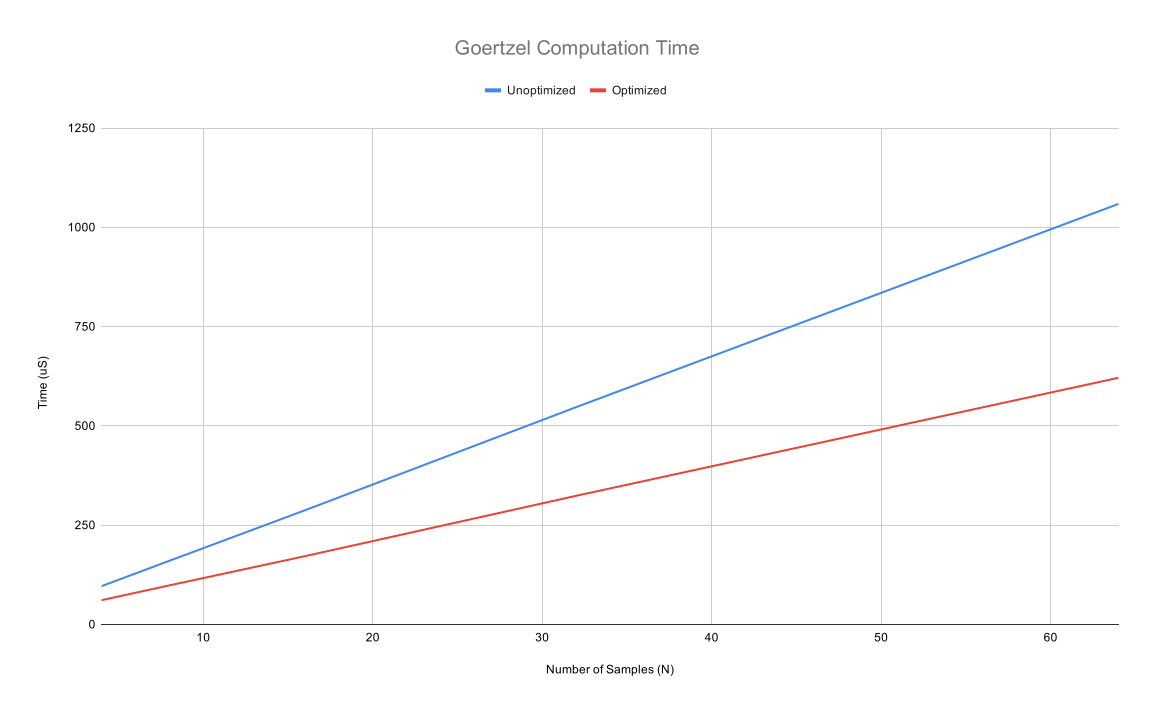
\includegraphics[width=\linewidth]{figures/results/goertzel_filter_speed/goertzel_computation_time.png}
	\captionof{figure}{Goertzel computation time versus sample set size}
	\label{fig:goertzel_computation_time}
\end{figure}

%\chapter{Discussion}
\label{ch_discussion}

%Here is what the results mean and how they tie to existing literature...

%Discuss the relevance of your results and how they fit into the theoretical work you described in your literature review.


\subsection{Focal Length of Lens}


\subsection{Light Focus System}


\subsection{Goertzel Filter Optimization}

Figure \ref{fig:goertzel_computation_plot} provides two important insights to the nature of the goertzel algorithm. The first observation may be found in the linearity of both plots, this confirms that both implementations of the algorithm have a time complexity of O(N) as noted in section \ref{sec:filter_optimization_design}. The practically perfect linearity in the results makes it possible to predict the timing requirements and make accurate theoretical predictions.

The gradient of the unoptimized curve is $16\mu S/sample$ and the gradient of the optimized curve is $9.3\mu S/sample$. The sampling rate used was $f_{sampling} \approx 144$kHz or $6.9\mu S/sample$. This indicates that even after optimizing the algorithm by simplifying out the multiplication step required for each new sample, the processor is still not fast enough to keep up with the rate of incoming samples.

The final observation is that the implemented optimization has two implications for the algorithms performance. The first implication is a small but non-zero constant timer saving, this comes as a result of removing the need for the multiplications to find the real and imaginary components of the k\textsubscript{th} DFT coefficient (see lines 18 and 19 of listing \ref{lst:goertzel_algorithm}). The second implication is a time difference which is directly proportional to the number of samples N, as indicated by the different gradients highlighted in the above paragraph.


\subsection{Goertzel Filter Performance}

\subsubsection{Simulated Frequency Response}

The simulation results shown in figure \ref{fig:goertzel_filter_response_simulated} reveal the familiar sinc function embedded in the frequency response curves. The form of these curves can be characterised by the $sinc^2(x)$ function which is to be expected because the filter returns the square of the magnitude.

It is clear from the plot that the filter is highly sensitive to the magnitude of the sampled waveform. A decrease in amplitude by a factor of two results in a four fold decrease in the amplitude of the filters response.




\subsubsection{Measured Frequency Response}

 %This is done in the results chapter
\chapter{Conclusions and Recommendations}
\label{ch_conclusions}

%These are the conclusions from the investivation and how the investigation changes things in this field or contributes to current knowledge...

%Draw suitable and intelligent conclusions from your results and subsequent discussion.

The core objective of this study was to develop a modular tagger-target system for the purposes of providing insight into the potential for more advanced laser tag systems that are robust to ambient lighting conditions and work over longer distances. In addition to this high level objective, this investigation set out to design and evaluate each module in the full system to provide a foundation for further research.

\section{Review of Modules}
Following the design, implementation and evaluation of the various modules, they have been categorized into two categories based on their performance. %Those categorized as having excellent performance are those that 

\subsection{Excellent Performance}

\textbf{Light Focus System}\\
The light focus system produced an optimal beam in the context of laser tag. The beam spot diameter at short distances less than 30m was less that 1m. This beam angle is the ideal size as it ensures some skill is required to aim the tagger while ensuring it isn't so challenging that it is impossible to make a single shot.

It was noted during the system test that for distances greater than 30m, the diameter of light detectable by the IR detectors was less than the the size predicted by the beam dispersion experiment. This effect worked to prevent the tagger from being too easy to aim at distant targets.

\textbf{Power LED Driver}\\
The power LED driver module had great performance. The linear current regulation resulted in very precise control over the timing and introduced very little noise into the system. In addition, by using a supply with a voltage close to that of the LED, very little heat was dissipated by the driving circuitry.

\textbf{IR Phototransistor Detector}\\
The IR phototransistor detector outperformed the photodiode detector because the amplification stage was robust to saturation caused by a large DC offset.

\textbf{IR Receiver}\\
The all in one package IR receiver outperformed the other IR detector modules, this was likely due to the built-in automatic gain control stage.

\textbf{Goertzel Filter}\\ %todo: I want to talk about speed of detection, but didn't do an experiemnt!!!
The digital tone decoder module exhibited exemplary performance. %todo: finnish this

\subsection{Adequate Performance}




%%%%%%%%%%%%%%%%%%%%

\section{Recommendations}

%recomend using a slightly larger lens

%implementing automatic gain control

%a superior microcontroller with DSP capabilities
\chapter{Recommendations}
\label{ch_recommendations}

%Make sensible recommendations for further work.

\include{bibtex/References}
\appendix
\chapter{Additional Files and Schematics}
\label{ch_appendixa}

%Add any information here that you would like to have in your project but is not necessary in the main
%text. Remember to refer to it in the main text. Separate your appendices based on what they are for
%example. Equation derivations in Appendix A and code in Appendix B etc.

\lstinputlisting[caption={Optimized Goertzel Algorithm - Octave Function\label{lst:optimized_goertzel_algorithm}}]{../goertzel/hc_calculate_goertzel.m}

\lstinputlisting[caption={Frequency Response Test - Octave Script\label{lst:frequency_response_script}}]{../goertzel/test_goertzel.m}

\begin{figure}[H]
	\centering
	\includegraphics[width=\linewidth]{figures/results/36khz_frequency.png}
	\caption{Plot of sampled 36kHz sinusoid}
	\label{fig:sampled_36khz_sinusoid}
\end{figure}

\begin{figure}[H]
	\centering
	\includegraphics[width=\linewidth]{figures/appendix/photodiode_0degrees.JPG}
	\caption{Output of photodiode module prior to full saturation}
	\label{fig:begin_saturation_of_photodiode}
\end{figure}
\chapter{Addenda}
\label{ch_addenda}

\section{GA Tracking Form}
\includepdf[pages=-]{appendix/ga_tracking_form.pdf}
\section{Ethics Forms}
\includepdf[pages=-, width=\textwidth]{appendix/ethics_form.pdf}
}
\end{document}
